\subsection{iOS}
I iOS applikationen designes view-klasser, der implementerer view-interfacet defineret i præsentationslaget. Det dominante user interface framework på iOS kaldes UIKit, og det er bygget op omkring en model-view-controller arkitektur. I UIKit har hvert view en tilhørende controller-klasse. I iOS designet tages der højde for dette, ved at bruge controller-klassen som en bro, i mellem Smartpools præsentationslag, og UIKits view-lag. Designet er derfor lavet således, at controller-klasserne på iOS implementerer view-interfacet fra præsentationslaget.

\subsubsection{SignUpViewBridge}
SignUpViewBridge-klassen implementerer ISignUpView interfacet. Klassen indeholder en række UIKit user interface elementer, som passer sammen med interfacet. Da dette view omhandler brugeroprettelse, er klassen designet til at indeholde en række tekstfelter, og en knap til at fuldende brugeroprettelsen. Denne klasse er designet til at nedarve fra UIKit klassen UIViewController, da de user interface elementer der indgår i designet, forventes at være statiske.

\begin{figure}
	\centering
	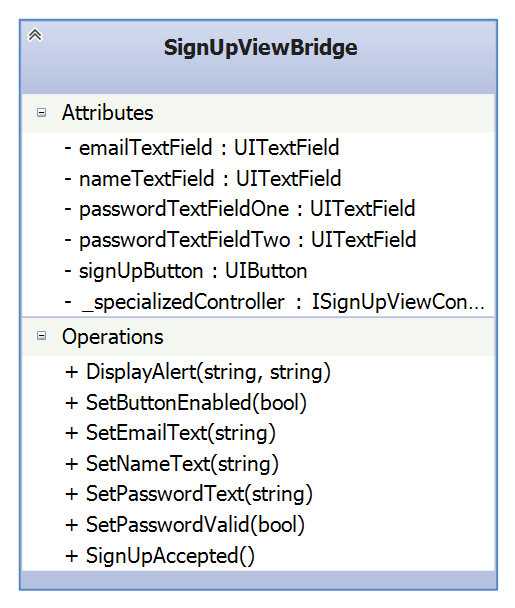
\includegraphics[width=0.3\linewidth]{figs/design/ios_signupviewbridge}
	\caption{SignUpViewBridge}
	\label{fig:ios_signupviewbridge}
\end{figure}

\subsubsection{StatViewBridge}
StatViewBridge-klassen implementerer IStatView interfacet. Dette view bør kunne håndtere dynamisk indlæsning og visning af måledata i følge de user stories, der er tilknyttet interfacet. Af denne grund nedarver StatViewBridge fra UITableViewController, der kan opsættes til at præsentere en dynamisk liste. StatViewBridge indeholder en UIBarButtonItem, der kan bruges til at skifte imellem pools i systemet.

\begin{figure}
	\centering
	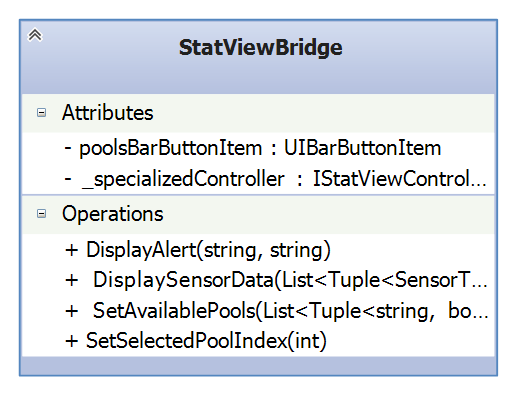
\includegraphics[width=0.3\linewidth]{figs/design/ios_statviewbridge}
	\caption{StatViewBridge}
	\label{fig:ios_statviewbridge}
\end{figure}
For yderligere forklaring se dokumentation afsnit Applikationslaget under Design.